
\documentclass[main.tex]{subfiles}
\begin{document}
\newcommand\coverwidth{0.093}

\twocolumn[{
\maketitle
\ssmall
\begin{center}
\begingroup
\setlength{\tabcolsep}{1pt}
\begin{tabular}{ccccccccccc}

\rotatebox[origin=c]{90}{\scriptsize{CIFAR-100}} &
    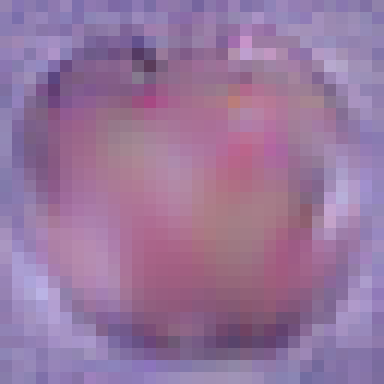
\includegraphics[align=c,width=\coverwidth\linewidth]{figures/cover/cifar/apple_0.pdf} &
    
\includegraphics[align=c,width=\coverwidth\linewidth]{figures/cover/cifar/camel_0.pdf} &
    
\includegraphics[align=c,width=\coverwidth\linewidth]{figures/cover/cifar/clock_0.pdf} &
    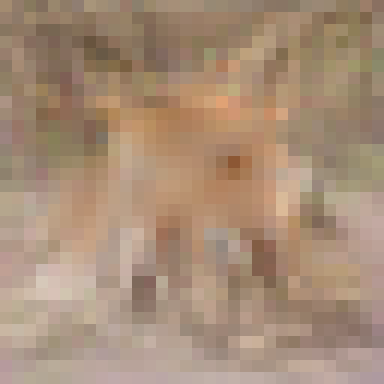
\includegraphics[align=c,width=\coverwidth\linewidth]{figures/cover/cifar/fox_0.pdf} &
    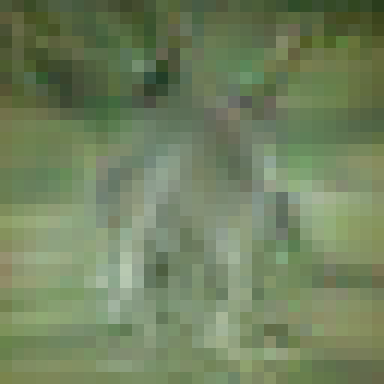
\includegraphics[align=c,width=\coverwidth\linewidth]{figures/cover/cifar/kangaroo_0.pdf} &
    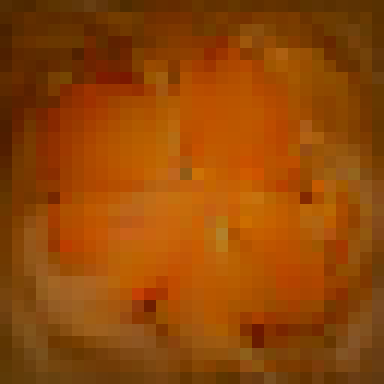
\includegraphics[align=c,width=\coverwidth\linewidth]{figures/cover/cifar/orange_0.pdf} &
    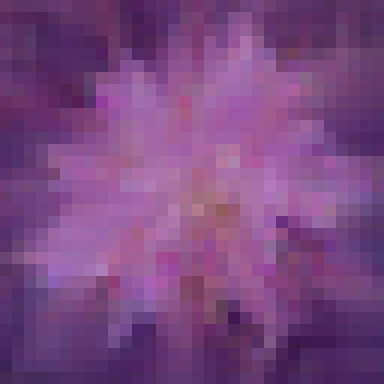
\includegraphics[align=c,width=\coverwidth\linewidth]{figures/cover/cifar/orchid_0.pdf} &
    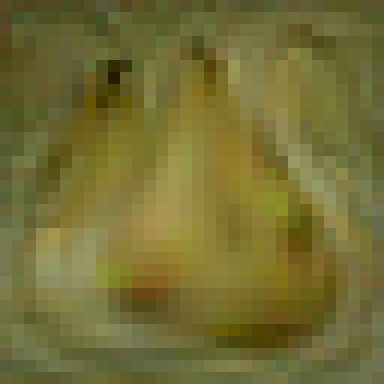
\includegraphics[align=c,width=\coverwidth\linewidth]{figures/cover/cifar/pear_0.pdf} &
    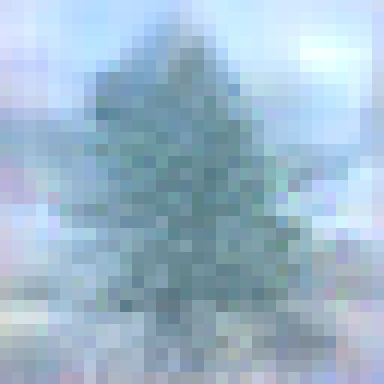
\includegraphics[align=c,width=\coverwidth\linewidth]{figures/cover/cifar/pine_tree_0.pdf} &
    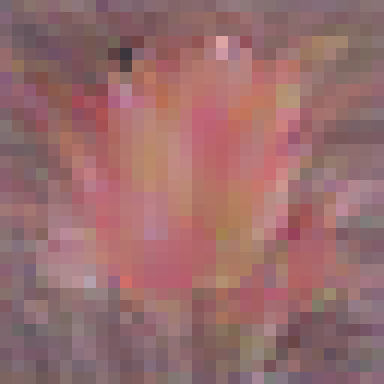
\includegraphics[align=c,width=\coverwidth\linewidth]{figures/cover/cifar/tulip_0.pdf} \\[7.8ex]
    & Apple & Camel & Clock & Fox & Kangaroo & Orange & Orchid & Pear & Pine Tree & Tulip\\[-0.15cm]\\
    \rotatebox[origin=c]{90}{\scriptsize{Tiny ImageNet}} &
    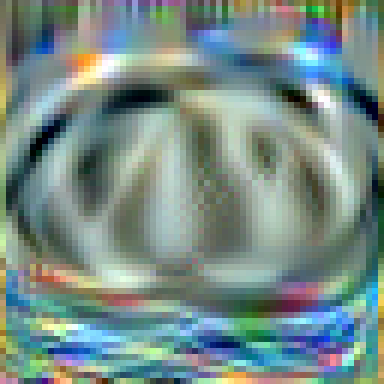
\includegraphics[align=c,width=\coverwidth\linewidth]{figures/cover/tiny/0_guinea_pig_0.pdf} &
    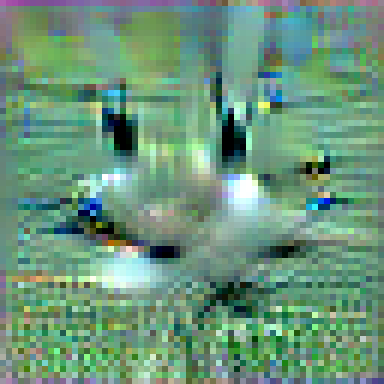
\includegraphics[align=c,width=\coverwidth\linewidth]{figures/cover/tiny/goose_0.pdf} &
    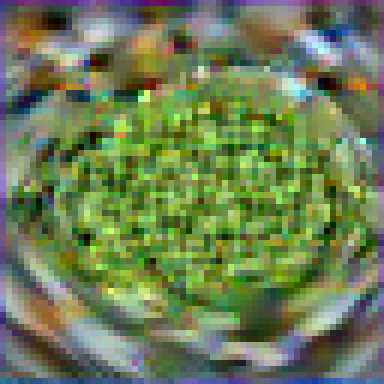
\includegraphics[align=c,width=\coverwidth\linewidth]{figures/cover/tiny/guacamole_0.pdf} &
    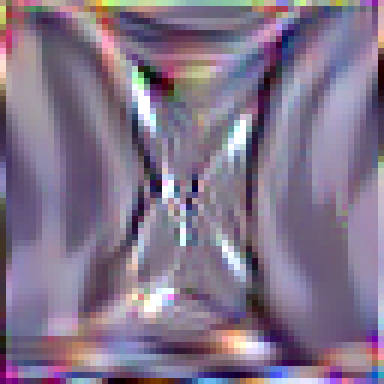
\includegraphics[align=c,width=\coverwidth\linewidth]{figures/cover/tiny/hourglass_0.pdf} &
    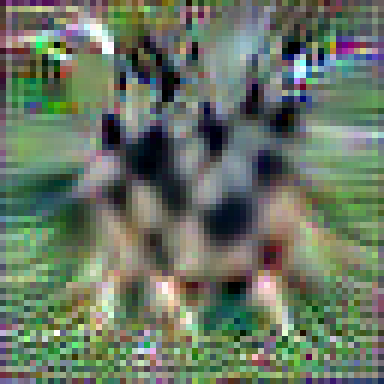
\includegraphics[align=c,width=\coverwidth\linewidth]{figures/cover/tiny/z_german_shepherd_0.pdf} &
    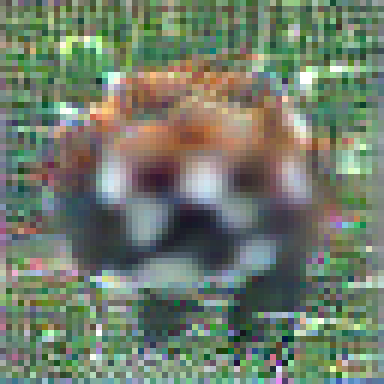
\includegraphics[align=c,width=\coverwidth\linewidth]{figures/cover/tiny/lesser_panda_0.pdf} &
    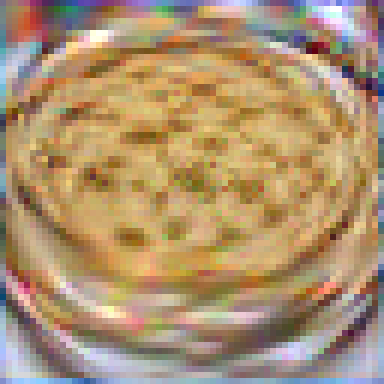
\includegraphics[align=c,width=\coverwidth\linewidth]{figures/cover/tiny/potpie_0.pdf} &
    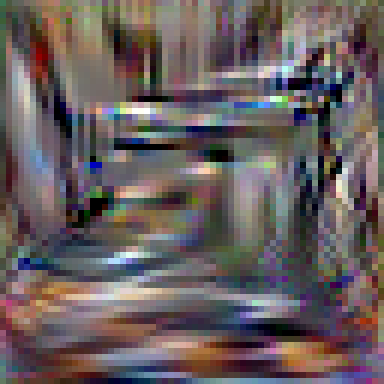
\includegraphics[align=c,width=\coverwidth\linewidth]{figures/cover/tiny/sewing_machine_0.pdf} &
    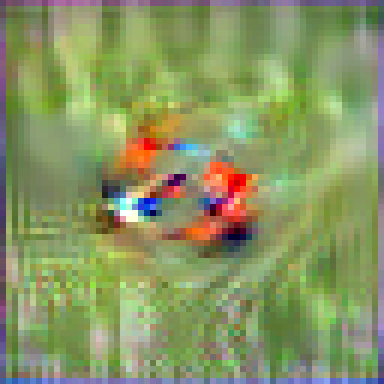
\includegraphics[align=c,width=\coverwidth\linewidth]{figures/cover/tiny/ladybug_0.pdf} &
    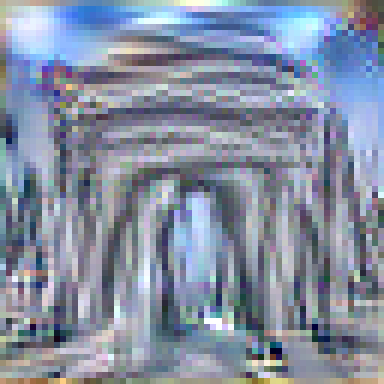
\includegraphics[align=c,width=\coverwidth\linewidth]{figures/cover/tiny/zz_triumphal_arch_0.pdf}\\[7.8ex]
    &Guinea Pig & Goose & Guacamole & Hourglass & German Shepard & Red Panda & Potpie & Sewing Machine & Ladybug & Triumphal Arch\\[-0.15cm]\\
    \rotatebox[origin=c]{90}{\scriptsize{ImageNet}} &
    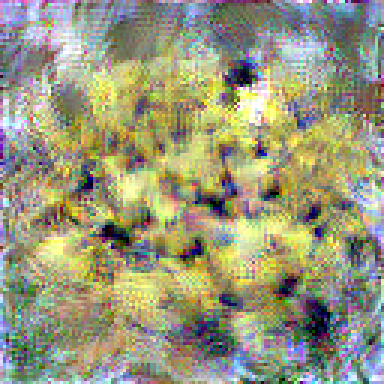
\includegraphics[align=c,width=\coverwidth\linewidth]{figures/cover/imagenet/banana_0.pdf} &
    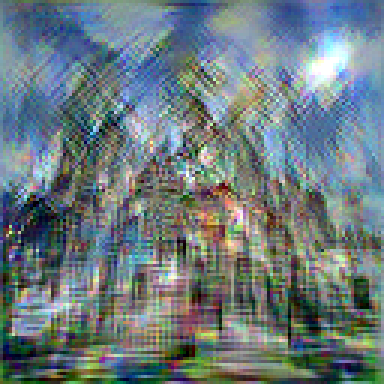
\includegraphics[align=c,width=\coverwidth\linewidth]{figures/cover/imagenet/church_0.pdf} &
    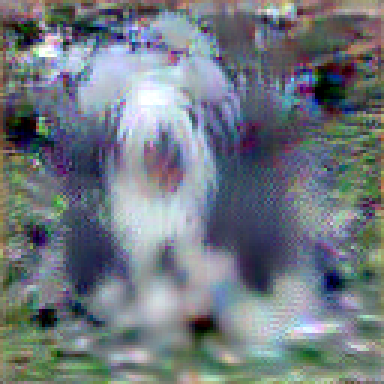
\includegraphics[align=c,width=\coverwidth\linewidth]{figures/cover/imagenet/english_sheepdog_0.pdf} &
    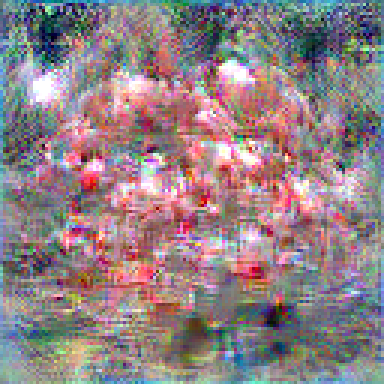
\includegraphics[align=c,width=\coverwidth\linewidth]{figures/cover/imagenet/flamingo_0.pdf} &
    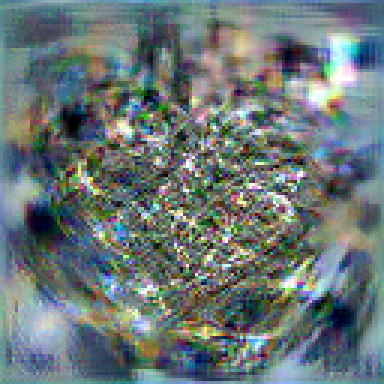
\includegraphics[align=c,width=\coverwidth\linewidth]{figures/cover/imagenet/french_horn_0.pdf} &
    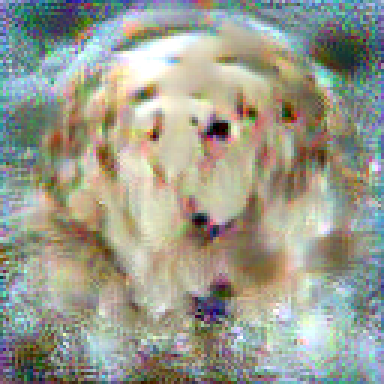
\includegraphics[align=c,width=\coverwidth\linewidth]{figures/cover/imagenet/golden_retriever_0.pdf} &
    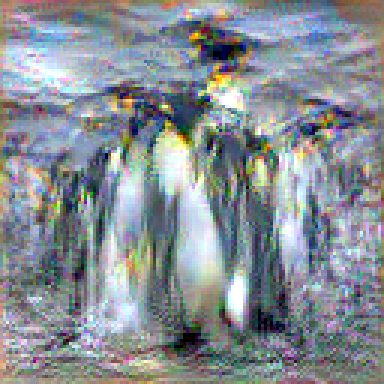
\includegraphics[align=c,width=\coverwidth\linewidth]{figures/cover/imagenet/king_penguin_0.pdf} &
    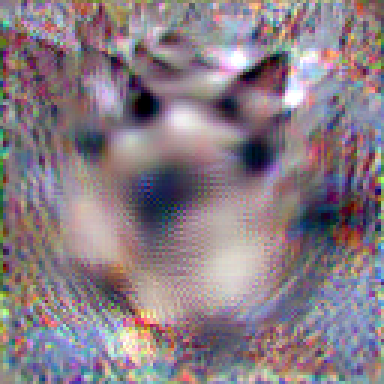
\includegraphics[align=c,width=\coverwidth\linewidth]{figures/cover/imagenet/siamese_cat_0.pdf} &
    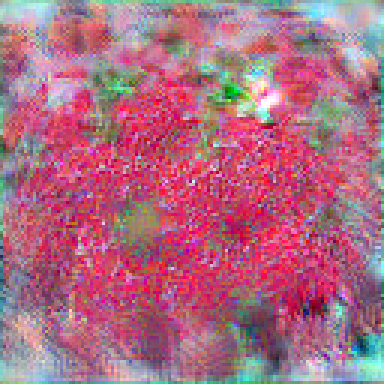
\includegraphics[align=c,width=\coverwidth\linewidth]{figures/cover/imagenet/strawberry_0.pdf} &
    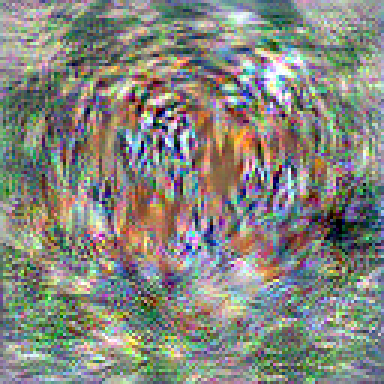
\includegraphics[align=c,width=\coverwidth\linewidth]{figures/cover/imagenet/tiger_0.pdf} \\[7.8ex]
    & Banana & Church & Sheepdog & Flamingo & French Horn & Golden Retriever & King Penguin & Siamese Cat & Strawberry & Tiger 
\end{tabular}
\endgroup\vspace{-0.25cm}
    \captionof{figure}{Example distilled images from 32x32 CIFAR-100 (top), 64x64 Tiny ImageNet (middle), and 128x128 ImageNet subsets (bottom). 
    Training a standard CNN using only such distilled images (as few as one per category) yields a trained model capable of test accuracy significantly better than previous methods of dataset distillation. Please see more results at \href{https://georgecazenavette.github.io/mtt-distillation/}{\color{blue}https://georgecazenavette.github.io/mtt-distillation/}.
    }
    \lblfig{teaser}
\end{center}
}]
\end{document}